\documentclass{article}

%Basics
\usepackage[margin=1in]{geometry}
\usepackage{amsmath, amssymb, amsthm}
\usepackage{enumitem}

%Drawing Graphs
\usepackage{tikz}

%Subfigures
\usepackage{subcaption}

%Multiple Columns
\usepackage{multicol}

%Formatting and Spacing
\setitemize[1]{noitemsep, parsep = 5pt, topsep = 5pt}
\setenumerate[1]{label = (\alph*), parsep = 1pt, topsep = 5pt}
\setlength\parindent{0pt}
\linespread{1.1}

%Easy Numbering
\newcounter{counter}
\newcommand{\Exercise}{Exercise \stepcounter{counter}\thecounter}

% %Custom Title Fields
\newcommand{\hmwkTitle}{Homework 5}
\newcommand{\hmwkDueDate}{March 12, 2022}
\newcommand{\hmwkClass}{Honors Discrete Mathematics}
\newcommand{\hmwkClassInstructor}{Professor Gerandy Brito}
\newcommand{\hmwkSection}{Spring 2022}
\newcommand{\hmwkAuthorName}{Sarthak Mohanty}

%Headers and Footers
\usepackage{fancyhdr}
\usepackage{extramarks}
\pagestyle{fancy}
\lhead{CS 2051}
\chead{\hmwkClass \ (\hmwkClassInstructor)}
\rhead{Homework 5}
\cfoot{\thepage}
\renewcommand\headrulewidth{0.4pt}
\renewcommand\footrulewidth{0.4pt}

\title{
    \vspace{1in}
    \textbf{\hmwkClass:\\ \hmwkTitle} \\
    \normalsize\vspace{0.1in}\small{Due\ on\ \hmwkDueDate\ at 11:59pm} \\
    \vspace{0.1in}\large{\textit{\hmwkClassInstructor\ \hmwkSection}} \\
    \vspace{1in}
    \begin{minipage}[t]{0.5\columnwidth}
    {\footnotesize You may collaborate with other students in this class, but (1) you must write up your own solutions in your own words, and (2) you must write down everyone you worked with at the top of the page, or ``no collaborators'' if you did it all on your own. Additionally, if you used any outside websites or textbooks besides the course text, please cite them here. You may not use question-answer sites like Chegg or MathOverflow.}
    \end{minipage}
    \vspace{1in}
    \author{\textbf{\hmwkAuthorName}}
    \date{}
}

\begin{document}
    
\maketitle
\pagebreak

\subsection*{Exercise 0 (Not Graded)}
About how many hours did you spend on this homework in total? Are there any topics that were particularly unclear that we should spend more time on?

\subsection*{\Exercise}
    Define a relation $\le_{i}$ on the Cartesian product $A_{1} \times A_{2} \times \cdots \times A_{n}$ as such: Given two sequences $(a_{n}) = (a_{1}, a_{2}, \dots, a_{n})$ and $(b_{n}) = (b_{1}, b_{2}, \dots, b_{n})$, declare that $(a_{n}) \le_{i} (b_{n})$ if and only if $a_{i} \le b_{i}$ for all $1 \le i \le n$.
    \begin{enumerate}
        \item Prove that this relation is a partial order.
        \item Let $Z = \{-3, -2, -1, 0, 1, 2, 3\}$. Draw a Hasse diagram corresponding to the poset $(Z \times Z, \le_{i})$. Briefly explain the general structure of this diagram if we were to extend the domain to all $\mathbb{Z} \times \mathbb{Z}$, and its similarity to the Cartesian plane.
        \item If we define this relation on the Cartesian product of $n$ totally ordered sets, is the relation a total order? Either prove or provide a counterexample.
    \end{enumerate}

\subsection*{\Exercise}
   \begin{enumerate}
       \item Draw the Hasse diagram of the poset $(D_{2470}, \mid)$, where $D_{n}$ is the set of all positive integers that divide $n$, and $\mid$ is the divisibility relation.
       \item Draw the Hasse diagram of the poset $(\mathcal{P}(\{2, 5, 19, 13\}), \subseteq)$. Explain the similarities between the Hasse diagram you just drew and the Hasse diagram in part (a), and the underlying relationship between the two posets causing these similarities.
       \item Without explicitly drawing the Hasse diagrams, explain the similarities between the Hasse diagrams of the posets $(D_{140}, \mid)$ and $(D_{525}, \mid)$, and the underlying relationship between the two posets causing these similarities.
       
       \vspace{1.5mm} {\small \textit{Hint: Consider using a similar (but not identical!) argument as in part (b).}}
   \end{enumerate}

\subsection*{\Exercise}
    A binary tree is a structure in which each node in the tree has at most two children nodes branching off of it, as shown in Figure \ref{fig:Q3}. A binary tree is \textit{full} if all of its nodes have either zero or two children. Let $B_{n}$ denote the number of full binary trees with $n$ nodes.
    
    \vspace{1.5mm}
    For $n > 1$, give a recurrence relation for $B_{n}$ (You do not have to find a closed form). Justify your answer.

    \begin{figure}[htbp]
        \centering
        \begin{subfigure}{.4\textwidth}
            \centering
            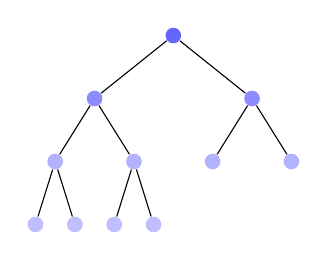
\begin{tikzpicture}
                [level distance=8mm,
                every node/.style={fill=blue!60,circle,inner sep=2pt},
                level 1/.style={sibling distance=20mm,nodes={fill=blue!45}},
                level 2/.style={sibling distance=10mm,nodes={fill=blue!30}},
                level 3/.style={sibling distance=5mm,nodes={fill=blue!25}}]
                \node {}
                child {node {}
                child {node {}
                child {node {}}
                child {node {}}
                }
                child {node {}
                child {node {}}
                child {node {}}
                }
                }
                child {node {}
                child {node {}
                }
                child {node {}}
                };
            \end{tikzpicture}
        \end{subfigure}
        \begin{subfigure}{.4\textwidth}
            \centering
            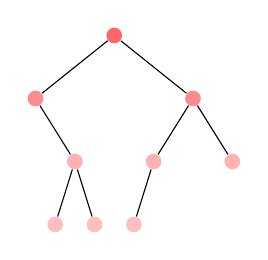
\begin{tikzpicture}
                [level distance=8mm,
                every node/.style={fill=red!60,circle,inner sep=2pt},
                level 1/.style={sibling distance=20mm,nodes={fill=red!45}},
                level 2/.style={sibling distance=10mm,nodes={fill=red!30}},
                level 3/.style={sibling distance=5mm,nodes={fill=red!25}}]
                \node {}
                child {node {}
                child[missing]
                child {node {}
                child {node {}}
                child {node {}}
                }
                }
                child {node {}
                child {node {}
                child {node {}}
                child[missing]
                }
                child {node {}}
                };
            \end{tikzpicture}
        \end{subfigure}
        \caption{Two examples of binary trees. The tree on the left is full, while the tree on the right is not.}
        \label{fig:Q3}
    \end{figure}

\subsection*{\Exercise}
    Use the method of your choice to solve the following recursions.
    \begin{enumerate}
        \item $T(n) = 5T(n - 1) - 8T(n - 2) + 4T(n - 3) \text{ where $T(0) = 1$, $T(1) = 0$, and $T(2) = 0$}.$
        \item $T(n) = 2T(n/2) + n\log(n) \text{ where } T(1) = c \text{ (here $c$ is a constant)}.$
    \end{enumerate}
    {\small Note: While you may use any of the methods discussed in class to solve these recurrences, in each part, there may be a method considered ``easier" than the other.}

\subsection*{\Exercise}
    In each part, as in lecture, start with the definition and get the values of $c$ and $k$.
    \begin{enumerate}
        \item Let $f, g$ be real functions satisfying $f = \mathcal{O}(g)$. Show that $a \cdot f = \mathcal{O}(g)$ for all $a \in \mathbb{R}^{*}$.
        \item Let $f_{1}, f_{2}, g$ be real functions satisfying $f_{1} = \mathcal{O}(g)$ and $f_{2} = \mathcal{O}(g)$. Show that $f_{1} + f_{2} = \mathcal{O}(g)$.
        \item Let $f_{1}, f_{2}, g_{1}, g_{2}$ be real functions satisfying $f_{1} = \mathcal{O}(g_{1})$ and $f_{2} = \mathcal{O}(g_{2})$. Show that $f_{1} \cdot f_{2} = \mathcal{O}(g_{1} \cdot g_{2})$.
    \end{enumerate}


\subsection*{\Exercise}
    Let $A$ be the set of all functions $f: \mathbb{N}^{+} \rightarrow \mathbb{R}^{+}$. Consider the relation $\sim$ on $A$ defined as follows: $$\text{$f \sim g$ if there exist constants $c_{1}, c_{2} > 0$ such that $c_{1}g(n) < f(n) < c_{2}g(n)$ for all $n \in \mathbb{N}^{+}$.}$$
    \begin{enumerate}
        \item Show that $\sim$ is an equivalence relation.
        \item It can similarly be shown that $\Theta$ is an equivalence relation. Group the following functions by equivalence classes such that functions $f(n)$ and $g(n)$ are in the same equivalence class iff $f = \Theta(g)$ (you do not need to show your work): 
        \begin{multicols}{4}
        \begin{itemize}
            \item $\log_{2}(n) + 1$
            \item $\log_{16}(n!)$
            \item $2n + 5$
            \item $(\log_{2}(n))^{\log_{2}(n)}$
            \item $n\log_{10}(n) + 1$
            \item $2021n + \log_{10}(n)$
            \item $2^{n}$
            \item $n^{1/\log_{6}(n)}$
            \item $3^{n}$
            \item $\ln(n^{2}) + 2021$
            \item $\frac{8n^{2} + 3n + 9}{n^{2}}$
            \item $n^{\log_{2}(\log_{2}(n))}$
        \end{itemize}
        \end{multicols}
    \end{enumerate}

\subsection*{\Exercise}
    \textit{(For this problem, you can use classical tools from Calculus such as $\epsilon-\delta$ definition of limits, derivatives, etc.)} Let $f, g$ be real functions with $f$ not identically zero and $g(x) \ne 0$ for all $x \in \mathbb{R}$ satisfying $$\lim_{x \rightarrow \infty} \left|\frac{f(x)}{g(x)}\right| = \ell.$$
    \begin{enumerate}
        \item Show that if $0 < \ell < \infty$, then $f = \Theta(g)$.
        \item Show that, if $l = 0$, then $f = \mathcal{O}(g)$. Give an example of functions for which $g \ne \mathcal{O}(f)$.
        \item Can you deduce a relation (of the form big-$\mathcal{O}$, big-$\Omega$, or big-$\Theta$) between $f$ and $g$ if $\ell = \infty$? Prove your answer.
        \item Let $p(x) = a_{n}x^{n} + a_{n - 1}x^{n - 1} + \dots + a_{1}x + a_{0}$ and $q(x) = b_{m}x^{m} + b_{m - 1}x^{m - 1} + \dots + b_{1}x + b_{0}$ be two polynomials with real coefficients. Use parts (a)--(c) to deduce when $p = \mathcal{O}(q)$, $p = \Omega(q)$, or $p = \Theta(q)$ (your answer should depend on $n$ and $m$).
    \end{enumerate}
\end{document}